\def\layersep{1.5cm}

\def\checkmark{\tikz\fill[scale=0.8, color=green_jon](0,.35) -- (.25,0) -- (1,.7) -- (.25,.15) -- cycle;} 
\definecolor{green_jon}{rgb}{0.0, 0.5, 0.0}

\begin{frame}{Geophysics Synthetic Example: Input Measurements}
\vspace{-0.35 cm}
\begin{figure}[H]
	\centering
	\begin{tikzpicture}[scale=1.0]
	\node (layers) at (0.0,0.0)[scale=0.7]{
		\begin{tikzpicture}

%% Tool
\fill[gray!80!white] (-1.5*3,0) -- (1.5*3,0.) --  node[right] {\small \bf \textcolor{black}{500 kHz}}  (1.5*3, 0.15*3) -- (-1.5*3,0.15*3) -- cycle;

%% Transmitters
\fill[black!80!white] (-0.6096*5-0.02*3,0) -- (-0.6096*5+0.02*3,0.) -- (-0.6096*5+0.02*3, 0.15*3) node[above] {\footnotesize \bf \textcolor{black}{Tx$_1$}}  -- (-0.6096*5-0.02*3,0.15*3) -- cycle;
%
\fill[black!80!white] (0.6096*5-0.02*3,0) -- (0.6096*5+0.02*3,0.)  -- (0.6096*5+0.02*3, 0.15*3) node[above] {\footnotesize \bf \textcolor{black}{Tx$_2$}} -- (0.6096*5-0.02*3,0.15*3) -- cycle;

%% Receivers
\fill[red!80!white] (-0.1016*5-0.02*3,0) -- (-0.1016*5+0.02*3,0.)  -- (-0.1016*5+0.02*3, 0.15*3) node[above] {\footnotesize \bf \textcolor{black}{Rx$_1$}} -- (-0.1016*5-0.02*3,0.15*3) -- cycle;
\fill[red!80!white] ( 0.1016*5-0.02*3,0) -- ( 0.1016*5+0.02*3,0.) -- ( 0.1016*5+0.02*3, 0.15*3)  node[above] {\footnotesize \bf \textcolor{black}{Rx$_2$}} -- ( 0.1016*5-0.02*3,0.15*3) -- cycle;

%% distances
\draw[black, line width=1pt,<->] (-0.1016*5, -0.6)      -- (0.1016*5, -0.6) node[pos=0.5, below] {\footnotesize \bf \textcolor{black}{0.40 m}}  ;
\draw[gray, dashed] (-0.1016*5, -0.6)      -- (-0.1016*5, 0)  ;
\draw[gray, dashed] ( 0.1016*5, -0.6)      -- ( 0.1016*5, 0)  ;

\draw[black, line width=1pt,<->] (-0.6096*5, -1.2)      -- (0.6096*5, -1.2) node[pos=0.5, below] {\footnotesize \bf \textcolor{black}{1.8 m}}  ;
\draw[gray, dashed] (-0.6096*5,-1.2)      -- (-0.6096*5, 0)  ;
\draw[gray, dashed] ( 0.6096*5,-1.2)      -- ( 0.6096*5, 0)  ;


\end{tikzpicture}
	};       
	\end{tikzpicture}
\end{figure}
\vspace{-0.7 cm}

	\begin{itemize}
		\item Co-axial attenuation and phase difference
	\end{itemize}
	
	\vspace{0.4 cm}

\begin{figure}[H]
	\centering
	\begin{tikzpicture}[scale=1.0]
	\node (layers) at (0.0,0.0)[scale=0.7]{
		\begin{tikzpicture}

%% Tool
\fill[gray!80!white] (-1.7*3,0) -- (1.7*3,0.) --  node[right] {\small \bf \textcolor{black}{10 kHz}}  (1.7*3, 0.15*3) -- (-1.7*3,0.15*3) -- cycle;

%% Transmitters
\fill[black!80!white] (-0.6096*5-0.02*3,0) -- (-0.6096*5+0.02*3,0.) -- (-0.6096*5+0.02*3, 0.15*3) node[above] {\footnotesize \bf \textcolor{black}{Tx}}  -- (-0.6096*5-0.02*3,0.15*3) -- cycle;
%
\fill[red!80!white] (0.6096*5-0.02*3,0) -- (0.6096*5+0.02*3,0.)  -- (0.6096*5+0.02*3, 0.15*3) node[above] {\footnotesize \bf \textcolor{black}{Rx}} -- (0.6096*5-0.02*3,0.15*3) -- cycle;

%% Receivers
%\fill[red!80!white] (-0.1016*5-0.02*3,0) -- (-0.1016*5+0.02*3,0.)  -- (-0.1016*5+0.02*3, 0.15*3) node[above] {\footnotesize \bf \textcolor{black}{Rx$_1$}} -- (-0.1016*5-0.02*3,0.15*3) -- cycle;
%\fill[red!80!white] ( 0.1016*5-0.02*3,0) -- ( 0.1016*5+0.02*3,0.) -- ( 0.1016*5+0.02*3, 0.15*3)  node[above] {\footnotesize \bf \textcolor{black}{Rx$_2$}} -- ( 0.1016*5-0.02*3,0.15*3) -- cycle;

%% distances
%\draw[black, line width=1pt,<->] (-0.1016*5, -0.6)      -- (0.1016*5, -0.6) node[pos=0.5, below] {\footnotesize \bf \textcolor{black}{0.40 m}}  ;
%\draw[gray, dashed] (-0.1016*5, -0.6)      -- (-0.1016*5, 0)  ;
%\draw[gray, dashed] ( 0.1016*5, -0.6)      -- ( 0.1016*5, 0)  ;

\draw[black, line width=1pt,<->] (-0.6096*5, -0.7)      -- (0.6096*5, -0.7) node[pos=0.5, below] {\footnotesize \bf \textcolor{black}{12 m}}  ;
\draw[gray, dashed] (-0.6096*5,-0.7)      -- (-0.6096*5, 0)  ;
\draw[gray, dashed] ( 0.6096*5,-0.7)      -- ( 0.6096*5, 0)  ;


\end{tikzpicture}
	};       
	\end{tikzpicture}
\end{figure}
\vspace{-0.7 cm}
	\begin{itemize}
		\item Co-axial attenuation and phase difference
		\item Geosignal
	\end{itemize}
\end{frame}


\begin{frame}{Geophysics Synthetic Example: Output Earth Parametrization}
\begin{columns}
    \begin{column}{0.35\textwidth}
    \begin{figure}[!h]
	\centering
	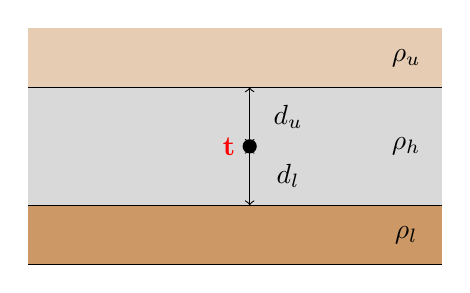
\begin{tikzpicture}[scale=1.5]
\draw (0,0) rectangle (3.5,2);

\fill[white!20!brown] (0,0) rectangle (3.5,0.5);
\fill[white!70!gray] (0,0.5) rectangle (3.5,1.5);
\fill[white!60!brown] (0,1.5) rectangle (3.5,2);


%\draw[red, line width=0.5 mm] (0.75,1.5) .. controls (1.15,1.1) .. (1.85,1) node (n1) at (0.85,1.6) {$\mathbf{t}$};
\draw[black, line width=0.1 mm] (0,0.5) -- (3.5,0.5);
\draw[black, line width=0.1 mm] (0,1.5) -- (3.5,1.5);

\fill[black] (1.875,1) circle (0.06cm);
\node (d_u) at (1.7,1) {\textcolor{red}{$\textbf{t}$}};
\draw[<->] (1.875,1.02) -- (1.875,1.5);
\node (d_u) at (2.2,1.25) {$d_u$}; 
\draw[<->] (1.875,0.98) -- (1.875,.5);
\node (d_u) at (2.2,0.75) {$d_l$};
\node (rho) at (3.2,1.75) {$\rho_u$};
\node (rho) at (3.2,0.25) {$\rho_l$};
\node (rho) at (3.2,1) {$\rho_h$};
\end{tikzpicture}

	\label{fig:param}
	\end{figure}
    \end{column}
    \begin{column}{0.5\textwidth}
        {\footnotesize $\rho_u \in [1,10^2] \Omega \cdot m$: Upper layer resistivity}\\
        \vspace{0.3cm}
        {\footnotesize $\rho_h \in [1,10^2] \Omega \cdot m$: Central layer resistivity}\\
        \vspace{0.3cm}
        {\footnotesize $\rho_l \in [1,10^2] \Omega \cdot m$: Lower layer resistivity}\\
        \vspace{0.3cm}
        {\footnotesize $d_u \in [10^{-2},10] m$: Vertical distance to upper layer}\\
        \vspace{0.3cm}
        {\footnotesize $d_l \in [10^{-2},10] m$: Vertical distance to lower layer}
    \end{column}
\end{columns}
\end{frame}



\begin{frame}{Synthetic Example}
\begin{center}
{\large Formation of model problem}
\end{center}
\begin{figure}
		\centering
		\pgfplotsset{every axis legend/.append style={
		at={(0.5,1.03)},
		anchor=south},
	every axis plot/.append style={line width=1.8pt},
}
\begin{tikzpicture}
\begin{axis}[
%  ymode=log,
%  xmode=log,
%  grid=both,
%xmin=0,
%xmax=540,
legend columns=2,
%  ymin=-20.0,
%  ymax=-11,
height=0.3*\textwidth,
width=0.85*\textwidth,
% 
y dir=reverse,
xlabel={HD ($m$)},
ylabel near ticks,
ylabel={TVD ($m$)},
%axis equal image,
enlargelimits=false,
]

%[enlargelimits=false, axis on top, axis equal image, width=6cm]

%\node[] at (rel axis cs:0,0) {\includegraphics{Syn_1/Predicted.png}};

\addplot graphics[xmin=0,xmax=540,ymin=45,ymax=60] {Diapos/DL_For_Inv/Figures/Syn_example/Numerical_results/Real.png};

\end{axis}	
\end{tikzpicture}

	%\caption{Formation of model problem}
	\label{fig:formation_model_1_original}
\end{figure}
\end{frame}


\begin{frame}{Encoder-Decoder Loss}
\begin{center}
Predicted formation
\end{center}
\begin{figure}
		\centering
		\pgfplotsset{every axis legend/.append style={
		at={(0.5,1.03)},
		anchor=south},
	every axis plot/.append style={line width=1.8pt},
}
\begin{tikzpicture}
\begin{axis}[
%  ymode=log,
%  xmode=log,
%  grid=both,
%xmin=0,
%xmax=540,
legend columns=2,
%  ymin=-20.0,
%  ymax=-11,
height=0.23*\textwidth,
width=0.75*\textwidth,
% 
 y dir=reverse,
xlabel={HD ($m$)},
ylabel near ticks,
ylabel={TVD ($m$)},
%axis equal image,
enlargelimits=false,
]

%[enlargelimits=false, axis on top, axis equal image, width=6cm]

%\node[] at (rel axis cs:0,0) {\includegraphics{Syn_1/Predicted.png}};

\addplot graphics[xmin=0,xmax=540,ymin=45,ymax=60] {Diapos/DL_For_Inv/Figures/Syn_example/Numerical_results/Enco-Deco/Predicted_F_FI.png};

\end{axis}	
\end{tikzpicture}

	%\caption{Formation of model problem}
	\label{fig:formation_model_1_original}
\end{figure}
\begin{center}
Geosignal measurement
\end{center}
\begin{figure}
		\centering
		\pgfplotsset{every axis legend/.append style={
		at={(0.5,1.03)},
		anchor=south},
	every axis plot/.append style={line width=1.8pt},
}
\begin{tikzpicture}
\begin{axis}[
%  ymode=log,
%  xmode=log,
%  grid=both,
xmin=0,
xmax=540,
legend columns=2,
%  ymin=-20.0,
%  ymax=-11,
height=0.23*\textwidth,
width=0.75*\textwidth,
%  y dir=reverse,
xlabel={HD ($m$)},
ylabel near ticks,
ylabel={Att. ($dB$)},
]
\addplot[blue,line width=1] table [x=X, y expr=(\thisrow{Atten_Geosignal} + 1.84)*8.68 ]{Diapos/DL_For_Inv/Figures/Syn_example/Numerical_results/Enco-Deco/F_aI_b.dat}
node[pos=0.8,inner sep=12pt, above,align=center,font=\linespread{1.0}\selectfont] { {\color{blue} ${\cal F} \circ {\cal I}$}
	{\color{black} vs} {\color{red} ${\cal F} \circ {\cal I}_{\theta^\ast}$}};

\addplot[red,dashed,line width=1] table [x=X, y expr=(\thisrow{Atten_Geosignal} + 1.84)*8.68 ]{Diapos/DL_For_Inv/Figures/Syn_example/Numerical_results/Enco-Deco/FI_b_without_regularization.dat};

\end{axis}	
\end{tikzpicture}

	%\caption{Formation of model problem}
	\label{fig:formation_model_1_original}
\end{figure}
\end{frame}


\begin{frame}{Encoder-Decoder Loss}
%\vspace{-0.5cm}
\begin{equation}
\begin{aligned}
	(\mathcal{F}_{\theta^\ast}, \mathcal{I}_{\phi^\ast}):=\arg \min_{\phi \in \Phi, \theta \in \Theta} \{ & \|(\mathcal{F}_{\theta} \circ \textcolor{blue}{\mathcal{I}_{\phi}})(\mathbf{M})-\mathbf{M}\| + \textcolor{green_jon}{\|{\cal F}_{\theta}({\bf P})-{\bf M}\|} \}
\end{aligned}
\notag
\end{equation}

\begin{figure}[!h]
	\centering
	\begin{tikzpicture}[scale=0.7]
\tikzset{cross/.style={cross out, draw=green_jon, minimum size=0.2cm, inner sep=0pt, outer sep=0pt},
%default radius will be 1pt. 
cross/.default={1pt}}

\draw (0,0) rectangle (8,4);
\node[left] at (0,4) {$\rho_l$};
\node[below] at (8,0) {$\rho_u$};

\draw (1,1) node[cross] {};
\draw (1,2) node[cross] {};
\draw (1,3) node[cross] {};

\draw (3,1) node[cross] {};
\draw (3,2) node[cross] {};
\draw (3,3) node[cross] {};

\draw (5,1) node[cross] {};
\draw (5,2) node[cross] {};
\draw (5,3) node[cross] {};

\draw (7,1) node[cross] {};
\draw (7,2) node[cross] {};
\draw (7,3) node[cross] {};

\draw (4,2) node[circle,draw=blue,minimum size=0.1cm] {};

\end{tikzpicture}



	\label{fig:regu}
\end{figure}

\center
\textcolor{green_jon}{x}=training samples

${\cal F}_\theta(\textcolor{green_jon}{x}) \approx {\cal F}(\textcolor{green_jon}{x})$

${\cal F}_\theta(\textcolor{blue}{O}) \neq {\cal F}(\textcolor{blue}{O})$
%\vspace{0.5cm}
\end{frame}


\begin{frame}{Two-Step Loss}
\begin{center}
Predicted formation
\end{center}
\begin{figure}[!h]
				\centering
	\pgfplotsset{every axis legend/.append style={
		at={(0.5,1.03)},
		anchor=south},
	every axis plot/.append style={line width=1.8pt},
}
\begin{tikzpicture}
\begin{axis}[
%  ymode=log,
%  xmode=log,
%  grid=both,
%xmin=0,
%xmax=540,
legend columns=2,
%  ymin=-20.0,
%  ymax=-11,
height=0.23*\textwidth,
width=0.75*\textwidth,
% 
 y dir=reverse,
xlabel={HD ($m$)},
ylabel near ticks,
ylabel={TVD ($m$)},
%axis equal image,
enlargelimits=false,
]

%[enlargelimits=false, axis on top, axis equal image, width=6cm]

%\node[] at (rel axis cs:0,0) {\includegraphics{Syn_1/Predicted.png}};

\addplot graphics[xmin=0,xmax=540,ymin=45,ymax=60] {Diapos/DL_For_Inv/Figures/Syn_example/Numerical_results/Two_Step/Predicted_F_FI_two_step.png};

\end{axis}	
\end{tikzpicture}
%
	%\caption{Predicted formation using the Encoder-Decoder loss function with regularization}
\end{figure}
\begin{center}
Geosignal measurement
\end{center}
\begin{figure}[!h]
	\centering
	\pgfplotsset{every axis legend/.append style={
		at={(0.5,1.03)},
		anchor=south},
	every axis plot/.append style={line width=1.8pt},
}
\begin{tikzpicture}
\begin{axis}[
%  ymode=log,
%  xmode=log,
%  grid=both,
xmin=0,
xmax=540,
legend columns=2,
%  ymin=-20.0,
%  ymax=-11,
height=0.23*\textwidth,
width=0.75*\textwidth,
%  y dir=reverse,
xlabel={HD ($m$)},
ylabel near ticks,
ylabel={Att. ($dB$)},
]
\addplot[blue,line width=1] table [x=X, y expr=(\thisrow{Atten_Geosignal} + 1.84)*8.68 ]{Diapos/DL_For_Inv/Figures/Syn_example/Numerical_results/Two_Step/F_aI_b.dat}
node[pos=0.8,inner sep=12pt, above,align=center,font=\linespread{1.0}\selectfont] { {\color{blue} ${\cal F} \circ {\cal I}$}
	{\color{black} vs} {\color{red} ${\cal F} \circ {\cal I}_{\theta^\ast}$}};

\addplot[red,dashed,line width=1] table [x=X, y expr=(\thisrow{Atten_Geosignal} + 1.84)*8.68 ]{Diapos/DL_For_Inv/Figures/Syn_example/Numerical_results/Two_Step/FI_b_two_step.dat};

\end{axis}	
\end{tikzpicture}
%
	%\caption{Deep coaxial measurement}
\end{figure}
\end{frame}


%==========================================================
\begin{frame}{Cross-plot}
\centering
\setlength{\fboxrule}{0.5mm}
\setlength{\fboxsep}{1mm}
\color{red}
\fbox{\parbox{3cm}{{\begin{align}
\textcolor{black}
{\mathcal{I} \hspace{0.25cm} vs \hspace{0.25cm} \mathcal{I}_{\phi^\ast}}
\notag
\end{align}}}}
\color{black}

$\qquad$ \\
\hspace{0.5cm} $d_u$ $\qquad \qquad \qquad \qquad \qquad$ $\rho_h$ $\qquad \qquad \qquad \qquad \qquad$ $\rho_u$
\begin{figure}[!h]
\centering
	{%
		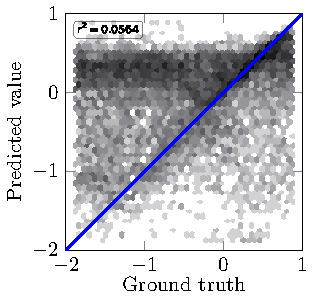
\includegraphics[scale=0.8]{Diapos/DL_For_Inv/Figures/Syn_example/Cross_plots/Two_Step_loss/C_P_4/d_u.pdf}
		\hspace{0.1cm}
		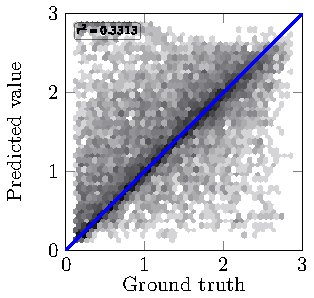
\includegraphics[scale=0.8]{Diapos/DL_For_Inv/Figures/Syn_example/Cross_plots/Two_Step_loss/C_P_4/rho_h.pdf}
		\hspace{0.1cm}
		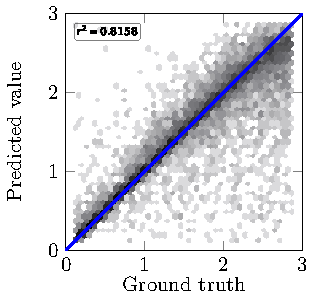
\includegraphics[scale=0.8]{Diapos/DL_For_Inv/Figures/Syn_example/Cross_plots/Two_Step_loss/C_P_4/rho_u.pdf}
		}	
\end{figure}	
\end{frame}


\begin{frame}{Encoder-Decoder Loss Regularization}
\begin{equation}
\begin{aligned}
	(\mathcal{F}_{\theta^\ast}, \mathcal{I}_{\phi^\ast}):=\arg \min_{\phi \in \Phi, \theta \in \Theta} \{ & \|(\mathcal{F}_{\theta} \circ \mathcal{I}_{\phi})(\mathbf{M})-\mathbf{M}\| +\|{\cal F}_{\theta}({\bf P})-{\bf M}\|\\
	&  + \textcolor{red}{\|{\cal I}_{\phi}({\bf M})-{\bf P}\| } \}
\end{aligned}
\notag
\end{equation} \\
\vspace{0.2cm}

\begin{figure}[!h]
				\centering
	\pgfplotsset{every axis legend/.append style={
		at={(0.5,1.03)},
		anchor=south},
	every axis plot/.append style={line width=1.8pt},
}
\begin{tikzpicture}
\begin{axis}[
%  ymode=log,
%  xmode=log,
%  grid=both,
%xmin=0,
%xmax=540,
legend columns=2,
%  ymin=-20.0,
%  ymax=-11,
height=0.23*\textwidth,
width=0.75*\textwidth,
% 
 y dir=reverse,
xlabel={HD ($m$)},
ylabel near ticks,
ylabel={TVD ($m$)},
%axis equal image,
enlargelimits=false,
]

%[enlargelimits=false, axis on top, axis equal image, width=6cm]

%\node[] at (rel axis cs:0,0) {\includegraphics{Syn_1/Predicted.png}};

\addplot graphics[xmin=0,xmax=540,ymin=45,ymax=60] {Diapos/DL_For_Inv/Figures/Syn_example/Numerical_results/Enco-Deco_REG/Predicted_F_FI_reg.png};

\end{axis}	
\end{tikzpicture}
%
	%\caption{Predicted formation using the Encoder-Decoder loss function with regularization}
\end{figure}

\begin{figure}[!h]
				\centering
	\pgfplotsset{every axis legend/.append style={
		at={(0.5,1.03)},
		anchor=south},
	every axis plot/.append style={line width=1.8pt},
}
\begin{tikzpicture}
\begin{axis}[
%  ymode=log,
%  xmode=log,
%  grid=both,
xmin=0,
xmax=540,
legend columns=2,
%  ymin=-20.0,
%  ymax=-11,
height=0.23*\textwidth,
width=0.75*\textwidth,
%  y dir=reverse,
xlabel={HD ($m$)},
ylabel near ticks,
ylabel={Att. ($dB$)},
]
\addplot[blue,line width=1] table [x=X, y expr=(\thisrow{Atten_Geosignal} + 1.84)*8.68 ]{Diapos/DL_For_Inv/Figures/Syn_example/Numerical_results/Enco-Deco_REG/F_aI_b.dat}
node[pos=0.8,inner sep=8pt, above,align=center,font=\linespread{1.0}\selectfont] { {\color{blue} ${\cal F} \circ {\cal I}$}
	{\color{black} vs} {\color{red} ${\cal F} \circ {\cal I}_{\theta^\ast}$}};

\addplot[red,dashed,line width=1] table [x=X, y expr=(\thisrow{Atten_Geosignal} + 1.84)*8.68 ]{Diapos/DL_For_Inv/Figures/Syn_example/Numerical_results/Enco-Deco_REG/FI_b.dat};

\end{axis}	
\end{tikzpicture}
%
	%\caption{Predicted formation using the Encoder-Decoder loss function with regularization}
\end{figure}
\end{frame}


\begin{frame}{Deep Learning for Inverse Borehole Problems}
\begin{itemize}
\item Deep Learning (DL) is an adequate option to invert borehole resistivity measurements in real time.
\vspace{0.5cm}
\item Traditional loss functions are not effective.
\vspace{0.5cm}
\item Both Encoder-Decoder and Two-Step are adequate alternatives.
\vspace{0.5cm}
\item Encoder-Decoder demands a regularization term.
\end{itemize}
\end{frame}